\chapter{Theoretical and phenomenological background}
\label{ch:background}
\graphicspath{{Chapter-Background/figures/}}

\section{Quantum chromodynamics}
\subsection{History and experimental motivation}

The atomic nucleus was discovered in the early 20th century \cite{Rutherford:1911zz}, and a few years later it was determined that it was composed of protons ($p$).
An additional, electrically-neutral nuclear constituent particle was proposed soon after and the neutron ($n$) was finally discovered in the early 1930s \cite{Chadwick:1932ma}.
Clearly some new type of interaction, strong enough to overcome electrostatic repulsion between protons, bound the nucleons ($p$ and $n$) together in the nucleus.
A particle field was proposed to mediate this strong interaction, dubbed the pion ($\pi^\pm$, $\pi^0$) \cite{Yukawa:1935xg}.
Since the strong interaction only acts over a length scale of about 2 fm, the mediating pion was predicted to have a mass of about 100 \MeV\footnote{The potential mediated by a boson of mass $m$ is proportional to \( - \exp(-mcr/\hbar)/r\), where $r$ is the separation between a pair of participants. Thus the mass of a mediating boson for a potential with a characteristic cutoff length of $\lambda$ is $m = \hbar/c\lambda = \frac{200 \MeVcc \textrm{fm}}{\lambda}$.}.
The charged pion was indeed discovered experimentally in 1947 \cite{Lattes:1947mw}.
Pions can be interpreted as the Nambu-Goldstone bosons corresponding to the spontaneously broken chiral symmetry, which explains their relatively small masses.

The expanding body of observed hadrons\footnote{a particle bound by the strong nuclear interaction} and their allowed decays suggested additional conserved quantum numbers suggested that they could be composed of constituent particles.
It was noticed that hadrons can be organized by their quantum numbers in a manner described by an $SU(3)$ \emph{flavor} symmetry \cite{GellMann:1962xb}.
This suggests that hadrons are composed of constituent particles called \emph{quarks}; however, the quark model was not immediately accepted because free quarks were not (and still have not been) observed.
Because electrons are point-like particles to the limits of current experiments, a scattering process $e^- A \rightarrow e^- X$ is dependent only on the internal structure of the target $A$.
The electron scatters through a virtual photon that interacts directly with the hadron in a process called \ac{DIS}\footnote{``deep'' because it probes the constituent structure of the target, ``inelastic'' because kinetic energy and matter are exchanged in the creation of the product particles}.

\begin{figure}[t]
  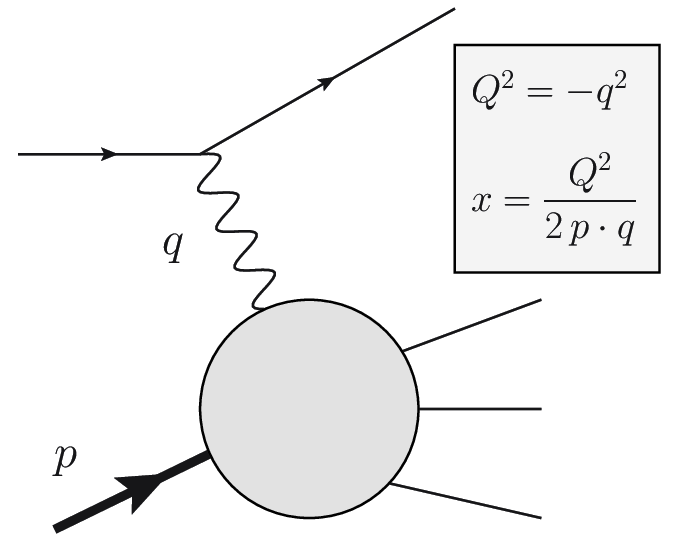
\includegraphics{dis_electron_proton.png}
  \caption{Deep inelastic scattering of a lepton on a hadron. Figure from \Ref{\cite{dis_fig_proceedings}}.
}
  \label{fig:dis}
\end{figure}

Under the constraints of Lorentz and gauge invariance, the cross-section of a \ac{DIS} process with incoming lepton and proton momenta $k$ and $P$ respectively and momentum transfer $q$ can be expressed as \cite{Tanabashi:2018oca}
\begin{equation}
  \frac{d^2 \sigma}{dx \, dQ^2} = \frac{4\pi\alpha^2_\textrm{EM}}{2xQ^4}\left[ \left(1+(1-y)^2\right) F_2\left(x, Q^2\right) - y^2 F_L \left(x, Q^2\right) \right]
  \label{eq:dis}
\end{equation}
where $Q^2 = -q^2$ is the absolute magnitude momentum transfer, $x = \frac{Q^2}{2q \cdot P}$, and $y = \frac{q \cdot P}{k \cdot P}$ is the fraction of the lepton's energy lost in the nucleon's rest frame.
In the parton model, $x$ is interpreted as the fraction of the target proton's momentum carried by a struck parton.
The structure functions $F_i(x, Q^2)$ describe the inherent internal structure of the proton.
The longitudinal structure function $F_L = F_2 - 2xF_1$ is zero by the Callan-Gross relation \cite{Callan:1969uq}, and experimentally the ratio $2xF_1 / F_2$ is consistent with 1 independent of $x$.
In the parton model, where the proton is described in terms of free point-like quarks constituents, the structure function $F_2$ is decomposed into \acp{PDF}
\begin{equation}
F_2 \left(x, Q^2\right) = x \sum_q e_q^2 f_{q/p}(x)
\end{equation}
to lowest order in the strong coupling constant $\alpha_s$.
The independence of $Q^2$ of the \acp{PDF} is a manifestation of their point-like description.
Higher-order corrections contribute variations in $Q^2$, as the scale of interactions between the quarks becomes relevant (\Cref{fig:proton_f2}).

\begin{figure}[t]
  %% page 326 of particle review
  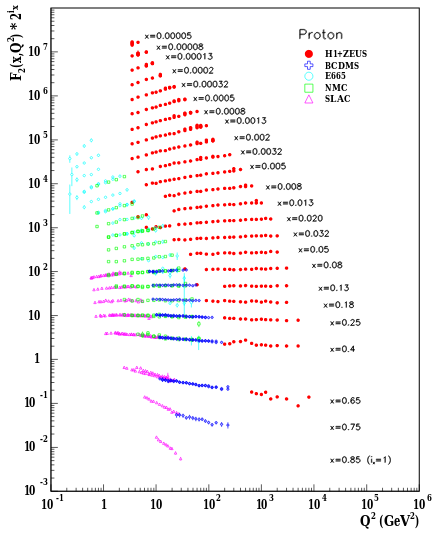
\includegraphics{proton_f2.png}
  \caption{The structure function $F_2\left(x, Q^2\right)$ of the proton.}
  \label{fig:proton_f2}
\end{figure}

%% motivated by the success of QED and SU(2) electroweak gauge theory, a gauge group of SU(3) color symmetry is a natural choice to attempt to describe the strong nuclear interaction.

\subsection{The QCD Lagrangian}
The lagrangian density of QCD is given by
\begin{equation}
  \Lagr_\mathrm{QCD} \equiv -\frac{1}{4} G^a_{\mu\nu}G^{a\mu\nu} + \bar{\psi} \left( i \slashed{D} - m \right) \psi \; .
\end{equation}
Here repeated indices are summed, where $\mu$ and $\nu$ indicate spacetime indices and $a$, $b$, and $c$ indicate color indices.
The covariant derivative
\[ D_\mu \equiv \partial_\mu - i g A^a_\mu t^a\]
where $A^a_\mu$ is the gluon field, $t^a$ are the generators of the $SU(3)$ gauge group, and $g$ is the coupling constant.
The gluon field strength tensor is
\[ G^a_{\mu\nu} \equiv \partial_\mu A^a_\nu - \partial_\nu A^a_\mu + g f^{abc} A^b_\mu A^c_\nu \]
with the $SU(3)$ structure constants defined such that
\[ [t^a,t^b] = if^{abc}t^c \; .\]
The quark fields are defined such that the mass matrix $m$ is diagonal:
\[ \bar{\psi}m\psi = \sum_{q = u,d,s,\ldots} m_{q}\bar{q}q \]
The quark masses $m_q$ are generated by the mechanism of spontaneous electro-weak symmetry breaking in which the Higgs field, coupling to fermions and electro-weak gauge bosons, acquires a nonzero vacuum expectation value.
This procedure induces a breaking of chiral symmetry $SU(N_f) \times SU(N_f) \rarrow SU(N_f)$ in the massless Lagrangian. %% reword. original lagrangian has chiral symmetry, but vacuum does not.

The QCD Lagrangian has a symmetry under the gauge transformation defined as...

\subsection{Running of the coupling constant} %% maybe doesn't deserve its own section
\subsection{Color confinement}
\subsection{Asymptotic freedom}

\section{QCD at high temperatures: the quark-gluon plasma}
\subsection{Experimental evidence for the existence of the QGP}
\subsection{Equation of state from lattice calculations}
\subsection{AdS-CFT correspondence}

\section{Hydrodynamic description of heavy ion collisions}
\subsection{Applicability of hydrodynamics}
low viscosity: large cross-section, low mfp
\subsection{Fourier decomposition of particle production}
\subsection{Success of hydrodynamics}
\subsection{Flow in small systems}

\section{Jet production and fragmentation}
Though the focus of this thesis is not on the physics of jet fragmentation, control of hard processes is essential to correctly extract observable quantities of interest.
This section will describe the physics behind jets.

TODO: Some of this discussion may be better moved elsewhere; for instance, nuclear modification may be appropriate in ``evidence for QGP''
\subsection{Parton model}
lorentz contraction in infinite momentum frame, transverse freeze-out, factorization
\subsection{Fragmentation function}
\subsection{Nuclear modification}


\section{Femtoscopy in heavy ion collisions}
This section will describe from a theoretical perspective what femtoscopy is and what it aims to achieve. The application of these techniques to experimental data will be addressed in \Cref{ch:analysis}.
\subsection{Imaging the source density function}
\subsection{Parameterization of the correlation function}
\subsection{Final-state interactions}
justify ignoring strong force; describe Coulomb correction (save jet fragmentation details for later)
\subsection{Motivation for femtoscopy in proton-lead}
\subsubsection{Collective expansion}

%% HI summary plots: (v2, RAA, etc)
%% https://atlas.web.cern.ch/Atlas/GROUPS/PHYSICS/CombinedSummaryPlots/HION/
